\documentclass{article}

%% MasteryNotebookTemplate.tex (c) by Emma Smith Zbarsky
%% MasteryNotebookTemplate.tex is licensed under a
%% Creative Commons Attribution 3.0 Unported License.

%%You should have received a copy of the license along with this
%%work.  If not, see <http://creativecommons.org/licenses/by/3.0/>.

\usepackage[usenames,dvipsnames]{color}
\usepackage{amssymb,amsmath, multirow}
\usepackage[initials]{amsrefs}
\usepackage{fullpage}
%\usepackage[all]{xy}
\usepackage{mathrsfs} %% for \mathscr and \mathfrak
\usepackage{graphicx} %% for \includegraphics

%% New stuff
\usepackage[pdftex,plainpages=false,hypertexnames=false,pdfpagelabels]{hyperref}
\usepackage{xcolor}
\definecolor{dark-red}{rgb}{0.7,0.25,0.25}
\definecolor{dark-blue}{rgb}{0.15,0.15,0.55}
\definecolor{medium-blue}{rgb}{0,0,0.65}
\hypersetup{
  colorlinks, linkcolor={purple},
  citecolor={medium-blue}, urlcolor={medium-blue}
}
%% End New Stuff

%\theoremstyle{hharemark}
\newtheorem{theorem}{Theorem}[section]
\newtheorem{proposition}[theorem]{Proposition}
\newtheorem{lemma}[theorem]{Lemma}
\newtheorem{corollary}[theorem]{Corollary}
\newtheorem{definition}[theorem]{Definition}
\newtheorem{assumption}[theorem]{Assumption}
\newtheorem{remark}{Remark}

\def\R{\mathbb{R}}
\def\Z{\mathbb{Z}}
\def\ds{\displaystyle}
\def\der#1#2{\frac{\partial #1}{\partial #2}} % partial derivatives
\def\d#1#2{\frac{d#1}{d#2}} % standard derivatives
\def\dt#1#2{\frac{d^2#1}{d#2^2}}
\def\dth#1#2{\frac{d^3#1}{d#2^3}}
\def\com#1{\texttt{#1}}
\def\x{\mathbf{x}}
\def\v{\mathbf{v}}
\def\bpm{\begin{pmatrix}}
\def\epm{\end{pmatrix}}
\def\O{\mathcal{O}}
\newcommand{\checked}{\makebox[0pt][l]{$\checkmark$}$\square$}
\newcommand{\unchecked}{$\Box$}
%\Theoremstyle{remark}

% Bernard Deconinck's macros
\newcommand{\beq}{\begin{equation}}
\newcommand{\eeq}{\end{equation}}
\newcommand{\ba}{\begin{array}}
\newcommand{\ea}{\end{array}}
\newcommand{\bea}{\begin{eqnarray*}}
\newcommand{\eea}{\end{eqnarray*}}
\newcommand{\bc}{\begin{center}}
\newcommand{\ec}{\end{center}}
\newcommand{\bt}{\begin{table}}
\newcommand{\et}{\end{table}}
\newcommand{\la}[1]{\label{#1}}
\newcommand{\p}{\partial}
\newcommand{\pp}[2]{{\partial #1 \over \partial #2}}
\newcommand{\ppn}[3]{{\partial^{#1} #2 \over \partial #3^{#1}}}
\newcommand{\mbf}[1]{\mbox{\boldmath {$#1$}}}
\newcommand{\red}[1]{\textcolor{red}{#1}}
\newcommand{\green}[1]{\textcolor{green}{#1}}
\newcommand{\blue}[1]{\textcolor{blue}{#1}}
\newcommand{\yellow}[1]{\textcolor{yellow}{#1}}
\newcommand{\purple}[1]{\textcolor{purple}{#1}}
\newcommand{\black}[1]{\textcolor{black}{#1}}

%\definecolor{RawSienna}{rgb}{.4,.2,0}

\begin{document}
\begin{titlepage}
  \begin{center}
    \bfseries
\huge Mastered Learning Objectives \\  from \\ Partial Differential Equations \\[.5in]
\large MATH 4900, Fall 2020 with Prof. Emma Zbarsky
\vfill
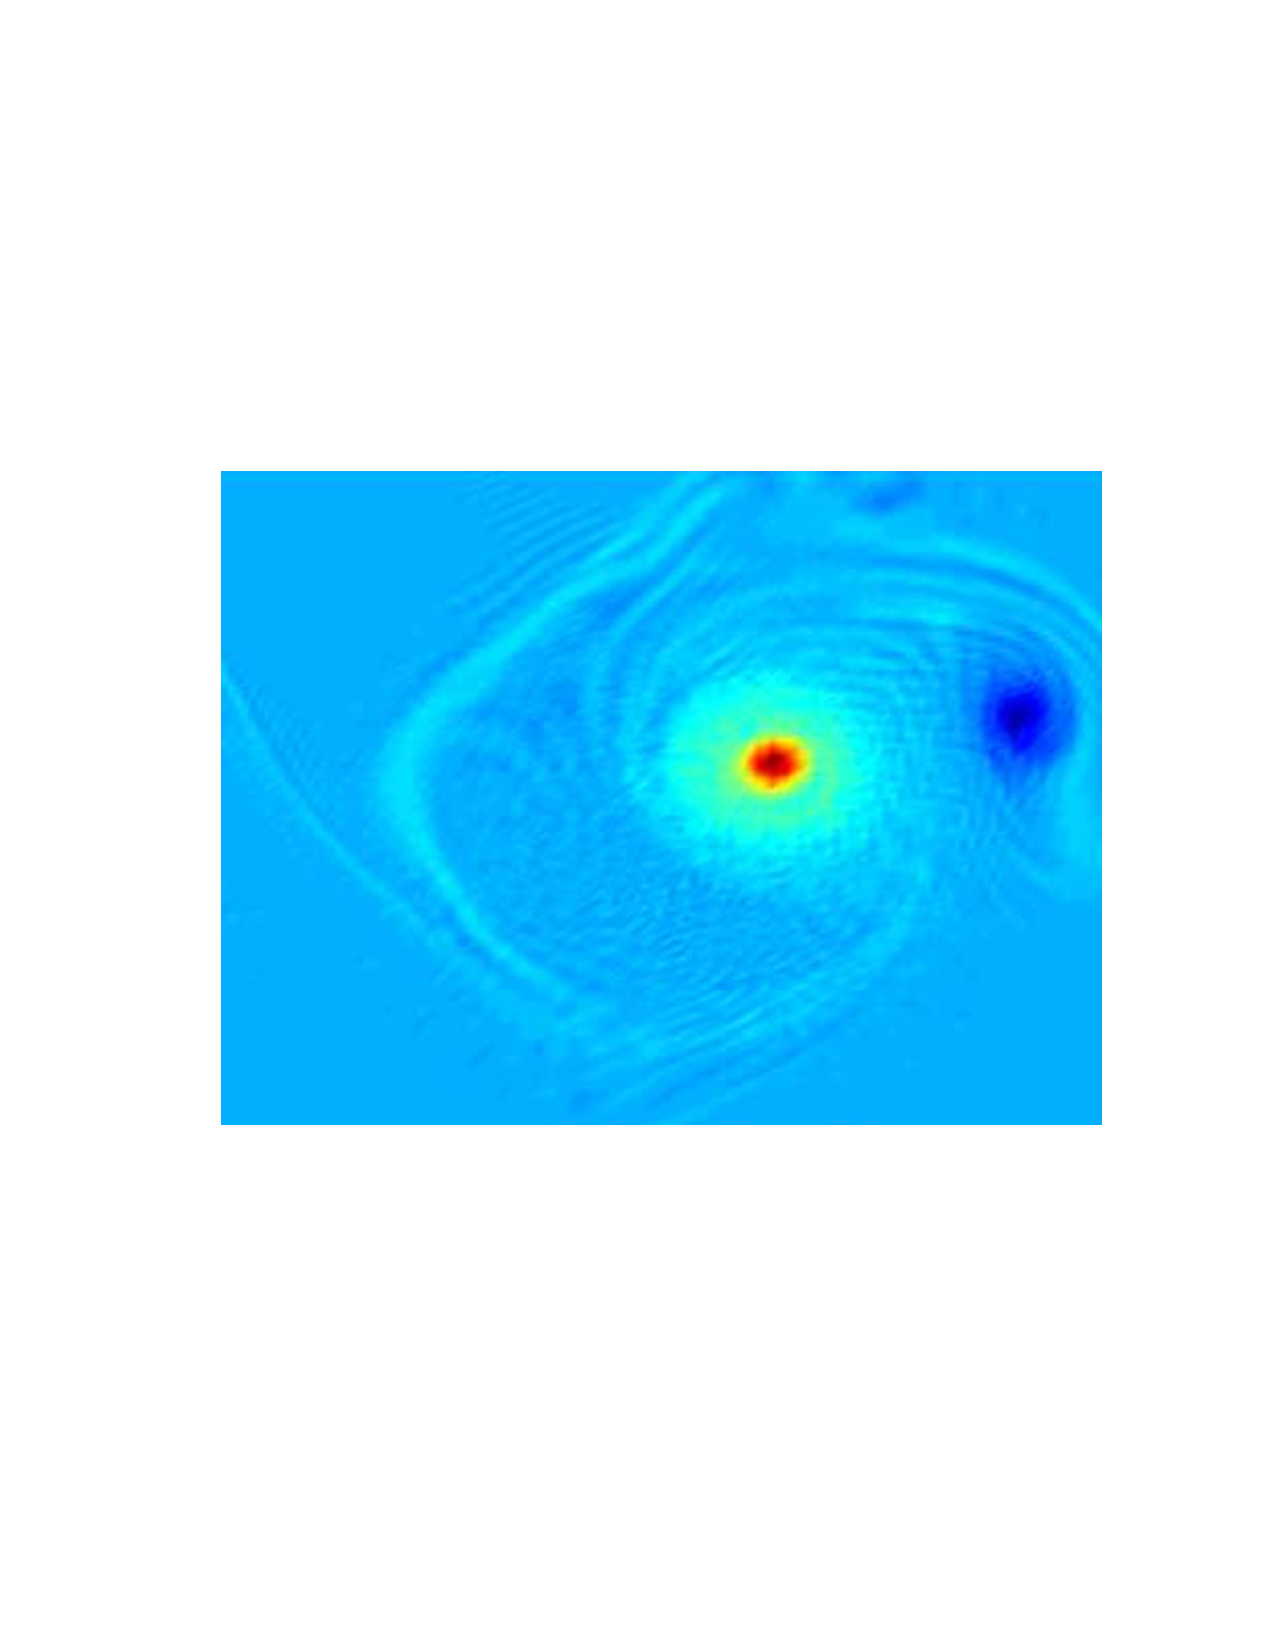
\includegraphics[height=3.5in, angle=90]{coolimage}
\vfill
\LARGE Your Name Here \\[.2in]
\texttt{youremailhere@wit.edu}
%\address{550 Huntington Ave,
%               Boston, MA 02115
%         USA}
%\thanks{You could thank grant support here.}
\end{center}      
\end{titlepage}
\newpage
\tableofcontents
\newpage

% Text of Document.  Use constructs such as \section, \subsection,
% \begin{theorem} ... \end{theorem}, \begin{proof} ... \end{proof}, etc.

\section{Mastery Check Planning}

% To check a box in the Productive Failure? column, replace the code \unchecked with \checked and recompile. 

\begin{tabular}{|l|c|c|c|c} \cline{1-4}
\multirow{2}{5cm}{\textbf{Standard}} & Suggested & Mastery Date & Writeup & Productive  \\ 
& Date & & Completed & Failure? \\ \cline{1-4}
\multirow{2}{5cm}{NM: Order of Error} & \multirow{2}{1.5cm}{Wk 2} &&& \multirow{2}{.4cm}{\unchecked} \\ &&&& \\ \cline{1-4}
\multirow{2}{5cm}{NM: Explicit Difference} & \multirow{2}{1.5cm}{Wk 3} &&& \multirow{2}{.4cm}{\unchecked} \\ &&&& \\ \cline{1-4}
\multirow{2}{5cm}{MC: Linear, constant speed}  & \multirow{2}{1.5cm}{Wk 3}&&& \multirow{2}{.4cm}{\unchecked} \\ &&&& \\ \cline{1-4}
\multirow{2}{5cm}{MC: Linear, polynomial speed} & \multirow{2}{1.5cm}{Wk 4}&&& \multirow{2}{.4cm}{\unchecked} \\ &&&& \\ \cline{1-4}
\multirow{2}{5cm}{MC: Nonlinear} &\multirow{2}{1.5cm}{Wk 4}&&& \multirow{2}{.4cm}{\unchecked} \\ &&&& \\ \cline{1-4}
\multirow{2}{5cm}{MC: Shock} &\multirow{2}{1.5cm}{Wk 5}&&& \multirow{2}{.4cm}{\unchecked} \\ &&&& \\ \cline{1-4}
\multirow{2}{5cm}{MC: Rarefaction} & \multirow{2}{1.5cm}{Wk 5}&&& \multirow{2}{.4cm}{\unchecked} \\ &&&& \\ \cline{1-4}
\multirow{2}{5cm}{NM: Neumann stability} &\multirow{2}{1.5cm}{Wk 6}&&& \multirow{2}{.4cm}{\unchecked} \\ &&&& \\ \cline{1-4}
\multirow{2}{5cm}{NM: CFL condition} &\multirow{2}{1.5cm}{Wk 6}&&& \multirow{2}{.4cm}{\unchecked} \\ &&&& \\ \cline{1-4}
\multirow{2}{5cm}{NM: Implicit Difference} &\multirow{2}{1.5cm}{Wk 6}&&& \multirow{2}{.4cm}{\unchecked} \\ &&&& \\ \cline{1-4}
\multirow{2}{5cm}{FS: Real Fourier Series} & \multirow{2}{1.5cm}{Wk 7} &&& \multirow{2}{.4cm}{\unchecked} \\ &&&& \\ \cline{1-4}
\multirow{2}{5cm}{FS: Complex Fourier Series} & \multirow{2}{1.5cm}{Wk 7} &&& \multirow{2}{.4cm}{\unchecked} \\ &&&& \\ \cline{1-4}
\multirow{2}{7cm}{FS: Convergence of Fourier Series} & \multirow{2}{1.5cm}{Wk 8} &&& \multirow{2}{.4cm}{\unchecked} \\ &&&& \\  \cline{1-4}
\multirow{2}{7cm}{FS: Integrability \& Differentiability of FS} & \multirow{2}{1.5cm}{Wk 8} &&& \multirow{2}{.4cm}{\unchecked} \\ &&&& \\  \cline{1-4}
\multirow{2}{5cm}{FS: Boundary Conditions} & \multirow{2}{1.5cm}{Wk 9} &&& \multirow{2}{.4cm}{\unchecked} \\ &&&& \\ \cline{1-4}
\multirow{2}{5cm}{SV: Heat Equation} & \multirow{2}{1.5cm}{Wk 10} &&& \multirow{2}{.4cm}{\unchecked} \\ &&&& \\ \cline{1-4}
\multirow{2}{5cm}{SV: Equilibrium behavior} & \multirow{2}{1.5cm}{Wk 10} &&& \multirow{2}{.4cm}{\unchecked} \\ &&&& \\ \cline{1-4}
\multirow{2}{5cm}{SV: Wave equation} & \multirow{2}{1.5cm}{Wk 11} &&& \multirow{2}{.4cm}{\unchecked} \\ &&&& \\ \cline{1-4}
\multirow{2}{5cm}{SV: d'Alembert's equation} & \multirow{2}{1.5cm}{Wk 12} &&& \multirow{2}{.4cm}{\unchecked} \\ &&&& \\ \cline{1-4}
\multirow{2}{5cm}{SV: Laplace equation} & \multirow{2}{1.5cm}{Wk 13} &&& \multirow{2}{.4cm}{\unchecked} \\ &&&& \\ \cline{1-4}
\multirow{2}{5cm}{Final Preparations} & \multirow{2}{1.8cm}{Wk 14/15} &&&   \\&&&& \\ \cline{1-4}
\end{tabular}
\newpage

%\section{Numerical Methods}
\section{Numerical Methods of Solving Partial Differential Equations}
\red{Give a brief overview of this section of the class. The following would be a sample introduction to such a section from an ordinary differential equations class.}
% Don't forget to delete all of the commentary and sample code before you submit this as your Mastery Notebook.

A first order initial value problem takes the form \(\ds \d{y}{t} = f(y,t)\) with \(\ds y(t_0)=y_0\). Such functions are studied in a first class on differential equations in a variety of special cases (e.g. separable equations or linear
equations) but there is no general analytic method that works for every \(f\). We shall explore some numerical methods of finding a solution.

\subsection{Order of Error}
\blue{Explain how you calculate the order of the error in a finite difference approximation scheme here. You should illustrate your explanation by solving at least the problem I gave you to demonstrate mastery. If you wish to include others as well that is up to you. What follows is a sample bit of text discussing the order of the error for the Euler Method of solving ODEs.}

The Euler Method takes the most basic ideas of calculus and uses them to step
through time to find an approximate solution.\\[.2in]
\begin{center}
\begin{tabular}{llcll}
Differential equation: & $\ds \d{y}{t} = f(y,t)$ &\phantom{aa} & 
Initial condition: & $y(t_0)=y_0$ \\
&&&& \\
Time interval of solution:& $[t_0, t_1]$ &&
Step size:& $\Delta t$ \\
&&&& \\
Number of steps:& $\ds \frac{t_1-t_0}{\Delta t}$ &&
Iterative step:& $\ds y(t+\Delta t) = f(y(t),t)\Delta
t+y(t)$ \end{tabular}\end{center}
~\\[.2in]

\subsubsection{Error} The error is of order $\Delta t$. In the limit as $\Delta t \to 0$, the error in Euler's
method also goes to 0. In practice, it is impractical to let $\Delta t$ become
too small as you reach limits in your computer's ability to resolve
numbers. You should check on the \emph{machine epsilon} \label{machineepsilon} for your computer and
the limitations of the data type you are using. This is also why you always want to add numbers
from the smallest to the largest on a computer as well to minimize the loss of
precision due to rounding.


\subsection{Neumann Stability}
\red{Explain the idea and solve the mastery problem that I gave you.}

 \subsection{The CFL Condition}
\blue{Explain the idea and solve the mastery problem that I gave you.}
 
\subsection{Implementing an Explicit Difference Method}
\red{Explain what an explicit difference method is. Explain what a boundary value problem is. Then present the sample problem from the text, with its solution, including reproductions of the graphs, and the sample problem you solved with me for mastery with its solution. Include your code here with clear explanations of what values must be changed to solve the two different problems. What follows is a sample MATLAB program that I wrote as an example of how to include commented code in a \LaTeX file.}

\begin{verbatim}
%% main_program.m
%%    Find the first 5 normalized eigenfunctions for Schrodinger's equation 
% %                   using the shooting method
clear variables; close all; clc

tol = 10^(-4);   % set the tolerance to work within

col=['r','b','g','c','m','k','y']; % eigenfunction colors

K = 1;                 % normalize to km/hbar^2 = 1
epsn = .9;             % define the initial parameter epsilon_n
psi=1;                 % define the initial guess for psi
L = 4;                 % range to work in
A = sqrt(L^2-epsn)*psi;   %left boundary differential
x0 = [psi A];          % provide the initial conditions x1(-4) = 1, x1'(-4) = 2
xp = -L:.1:L;          % define the span of the computational domain

eigvalues = zeros(5,1);              % define the results matrices
eigfunctions = zeros(length(xp),5);


epsilon_start = epsn;    % beginning value of epsilon

for modes = 1:5              % begin mode loop
    epsilon = epsilon_start; % initial value of eigenvalue epsilon
    deps = .05;              % default step size in epsilon
    for j = 1:1000           % begin convergence loop for epsilon
        x0 = [psi sqrt(L^2 - epsilon)*psi]; % Update initial condition for our new epsilon
        [t,y] = ode45(@(t,y) schrodinger(t,y,K,epsilon), xp, x0); % solve ODEs
        % Are we within tolerance?
        if (abs(-sqrt(L^2-epsilon)*y(end,1)-y(end,2))<tol)
            break                       % get out of convergence loop
        end
        % here we check to see if epsilon needs to be higher or lower
        % then we bisect to get closer to our required tolerance
        if (-1)^(modes)*(-sqrt(L^2-epsilon)*y(end,1)-y(end,2))>0     
            epsilon = epsilon+deps;    
        else
            epsilon = epsilon - deps/2;
            deps = deps/2;
        end                             % end bisection loop
    end                % end convergence loop
    
    eigvalues(modes) = epsilon;
    epsilon_start = epsilon+.1;    % after finding eigenvalue, pick
                                    % new starting value for next higher
                                    % mode
    norm = trapz(t,y(:,1).*y(:,1));    % calculates the normalization
    
    if modes > 0
    plot(t,y(:,1)/sqrt(norm),col(modes)); hold on   % plot modes
    end
    
    eigfunctions(:,modes) = y(:,1)/sqrt(norm);
    
end        % end modes loop
\end{verbatim}

\subsection{Implementing an Implicit Difference Method}
\blue{Explain what an implicit difference method is. Then present the sample problem from the text, with its solution and the sample problem you solved with me for mastery with its solution. Include your code here with clear explanations of what values must be changed to solve the two different problems. What follows is a sample using a block quotation and reference.}

J. D. Lambert described the phenomenon of stiffness for a system of
differential equations as follows:
\begin{quote} If a numerical method with a finite region of absolute stability,
    applied to a system with any initial conditions, is forced to use in a
    certain interval of integration a steplength which is excessively small in
    relation to the smoothness of the exact solution in that interval, then the
    system is said to be stiff in that interval. \cite{wikistiff}
    \end{quote}

\section{Method of Characteristics}
\red{Give an introduction to the method of characteristics.}

\subsection{Solving $u_t+cu_x +du = g(x)$ with $u(0,x)=f(x)$}
\blue{Explain how to solve such a problem when $c$ and $d$ are constants. Then present your solution to the mastery problem I gave you.}

\subsection{Solving the linear transport equation with polynomial coefficients}
\red{Explain how to solve such a problem when the wave speed is polynomial in $t$ or polynomial in $x$. Then demonstrate the solution with the mastery problem I gave you to solve.}

\subsection{Solving first order nonlinear PDEs using the method of characteristics}
\blue{Explain how to solve a problem of the form $u_t+g(u)u_x=0$. Then solve the mastery problem I gave you to solve. What follows is a sample use of equation array and piecewise defined functions.}
  \bea
y_{n+1} &=& y_n+\red{e} + \Delta t \lambda y_{n+1} \\
\left(1-\Delta t
\lambda\right)^ny_{n+1} &=& y_n+\red{e} \\
y_{n+1} &=& \left(\frac{1}{1-\Delta t \lambda}\right)(y_n+\red{e}) \\
y_{n+1} &=& \left(\frac{1}{1-\Delta t \lambda}\right)^{n+1}(y_0+\red{e}) 
\eea
and hence a global error after $N$ steps of
$$E = \left(\frac{1}{1-\Delta t \lambda}\right)^N\red{e}.$$ Therefore
$$\lim_{N\to \infty} E = \begin{cases} \infty & 
  |1-\Delta t \lambda|<1 \\
 0 &  |1-\Delta t \lambda|>1 \\
  \red{e} & |1-\Delta t \lambda|=1
  \end{cases}.$$


\subsection{Shocks}
\red{Explain how to recognize and solve a first order differential equation whose solution will involve a shock. Then solve the mastery problem I gave you. What follows is sample code for including a figure, Figure~\ref{fig:example}, with a caption and label.}
\begin{figure}[ht]
\begin{center}
  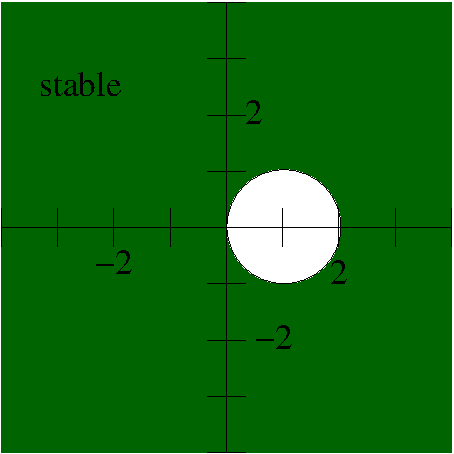
\includegraphics[width=2.5in]{stability-backwardeuler}
  \end{center}
\caption{Stable regions for forward (left) and backward (right) Euler methods where green is
  convergent and white is divergent. \label{fig:example}}
\end{figure}


\subsection{Rarefaction Waves}
\blue{Explain how to recognize and solve a first order differential equation that will result in a rarefaction wave. Then solve the mastery problem I gave you. What follows is sample code for a table. I have left some horizontal and vertical lines out for demonstration purposes, and doubled others.}
\begin{center}
\begin{tabular}{|l|ccc|} \hline
\textbf{Command} & \textbf{Local Error} & \textbf{Global Error} & \textbf{Scheme} \\ \hline \hline  
  \texttt{ode23} & $O(\Delta t^3)$ & $O(\Delta t^2)$ & Runge-Kutta\\
  \texttt{ode45} & $O(\Delta t^5)$ & $O(\Delta t^4)$ & Runge-Kutta \\ \hline
  \texttt{ode15s} & variable  & variable & Gear's method, stiff\\
  \texttt{ode113} & variable & variable & predictor/corrector \\ \hline
  \end{tabular}
  \end{center}
For more information, see the Matlab documentation \cite{matlabode}.

\section{Fourier Series}
\blue{Give an introduction to Fourier series.}

\subsection{Real Fourier Series}
\red{Explain how to calculate the real Fourier series for a suitable function. Then present the example that you solved for your mastery check.}

\subsection{Complex Fourier Series}
\blue{Explain how to calculate the complex Fourier series for a suitable function. Then present the example that you solved for your mastery check.}

\subsection{Convergence of Fourier Series}
\red{Discuss the convergence of Fourier series. Then present the example that you solved for your mastery check.}

\subsection{Integrability and Differentiability of Fourier Series}
\blue{Discuss the integrability and differentiability of Fourier series. Then present the example that you solved for your mastery check.}

\subsection{Boundary Conditions}
\red{Discuss the various standard types of boundary conditions and what conditions tell you about the form of a Fourier Series solution. Then present the example that you solved for your mastery check.}


\section{Separation of Variables}
\red{Give an overview of the method of separation of variables.}

\subsection{Equilibrium behavior of a solution}
\red{Explain what equilibrium behavior is and how one goes about finding the equilibrium behavior of a system. Then give the example that you solved for your mastery check.}

\subsection{Solving the 1D heat equation}
\blue{Explain how to solve the 1D heat equation with boundary conditions using the method of separation of variables. Then present the example that you solved for your mastery check.}

\subsection{Solving the Laplace equation}
\red{Explain how to solve the Laplace equation with boundary conditions using the method of separation of variables. Then present the example that you solved for your mastery check.}

\subsection{Solving the 1D wave equation}
\red{Explain how to solve the 1D wave equation with boundary conditions using the method of separation of variables. Then present the example that you solved for your mastery check.}

\subsection{Solving the 1D wave equation using d'Alembert's formula}
\red{Explain how to solve the 1D wave equation with boundary conditions using d'Alembert's formula. Then present the example that you solved for your mastery check.}


%\section{Bibliography}
\begin{bibdiv}
\begin{biblist}

\bibselect{numerical}

\end{biblist}
\end{bibdiv}

\end{document}
